\section{Evaluation}
\label{sec:evaluation}
\label{Simulation Result}
\subsection{Basic Setting and Description}
\indent 
	We conduct a simulation using the procedure described above. We put four robots in the simulation field and draw three range, representing the sensory range, communication range, and rejection range, for each robots. We draw straight lines between robots with the average signal strength of four antenna of robots between them instead of the signal strength of each robots for a better visualization. In this simulation we assumed following:
\begin{itemize}
	\item The frequency of the transceiver is at 2.4 Gigahertz range.
	\item Each robots is using different frequency channel so that each signal cannot interfere another.
	\item The reference distance of the transceiver is 1.8 meters and the receiving power at the reference distance is -27.25 decibel. The standard deviation of the Gaussian white noise is 1, since we do not know the real antenna's Signal-to-Noise Ratio.
	\item The sensory range, the communication range, and the rejection range are 200 meters, 100 meters, and 20 meters respectively.
\end{itemize}



\subsection{Signal Strength Analysis}
\par
	The sample results of the simulation are the following figures: figure 9 and figure 10. Figure 10 shows the signal strength against distance to visualize the relationship between signal strength and distance. Asides from the effect of the White Gaussian Noise and the Fading, it shows that it has a logarithmic relationship. Figure 9 shows four simulation results that the four robots are randomly placed and the average signal strength are measured accordingly. The simulation result in figure 9 shows that the measured average signal strength are measured differently with distance. It also shows that the robots around the communication range has signal strength around -60db, and the robots within the sensory range have signal strength of more than -70db, whereas the signal strength between two robots outside of the sensory range is measured less than -70db. \\
 
\begin{figure}[ht]
	\centering
	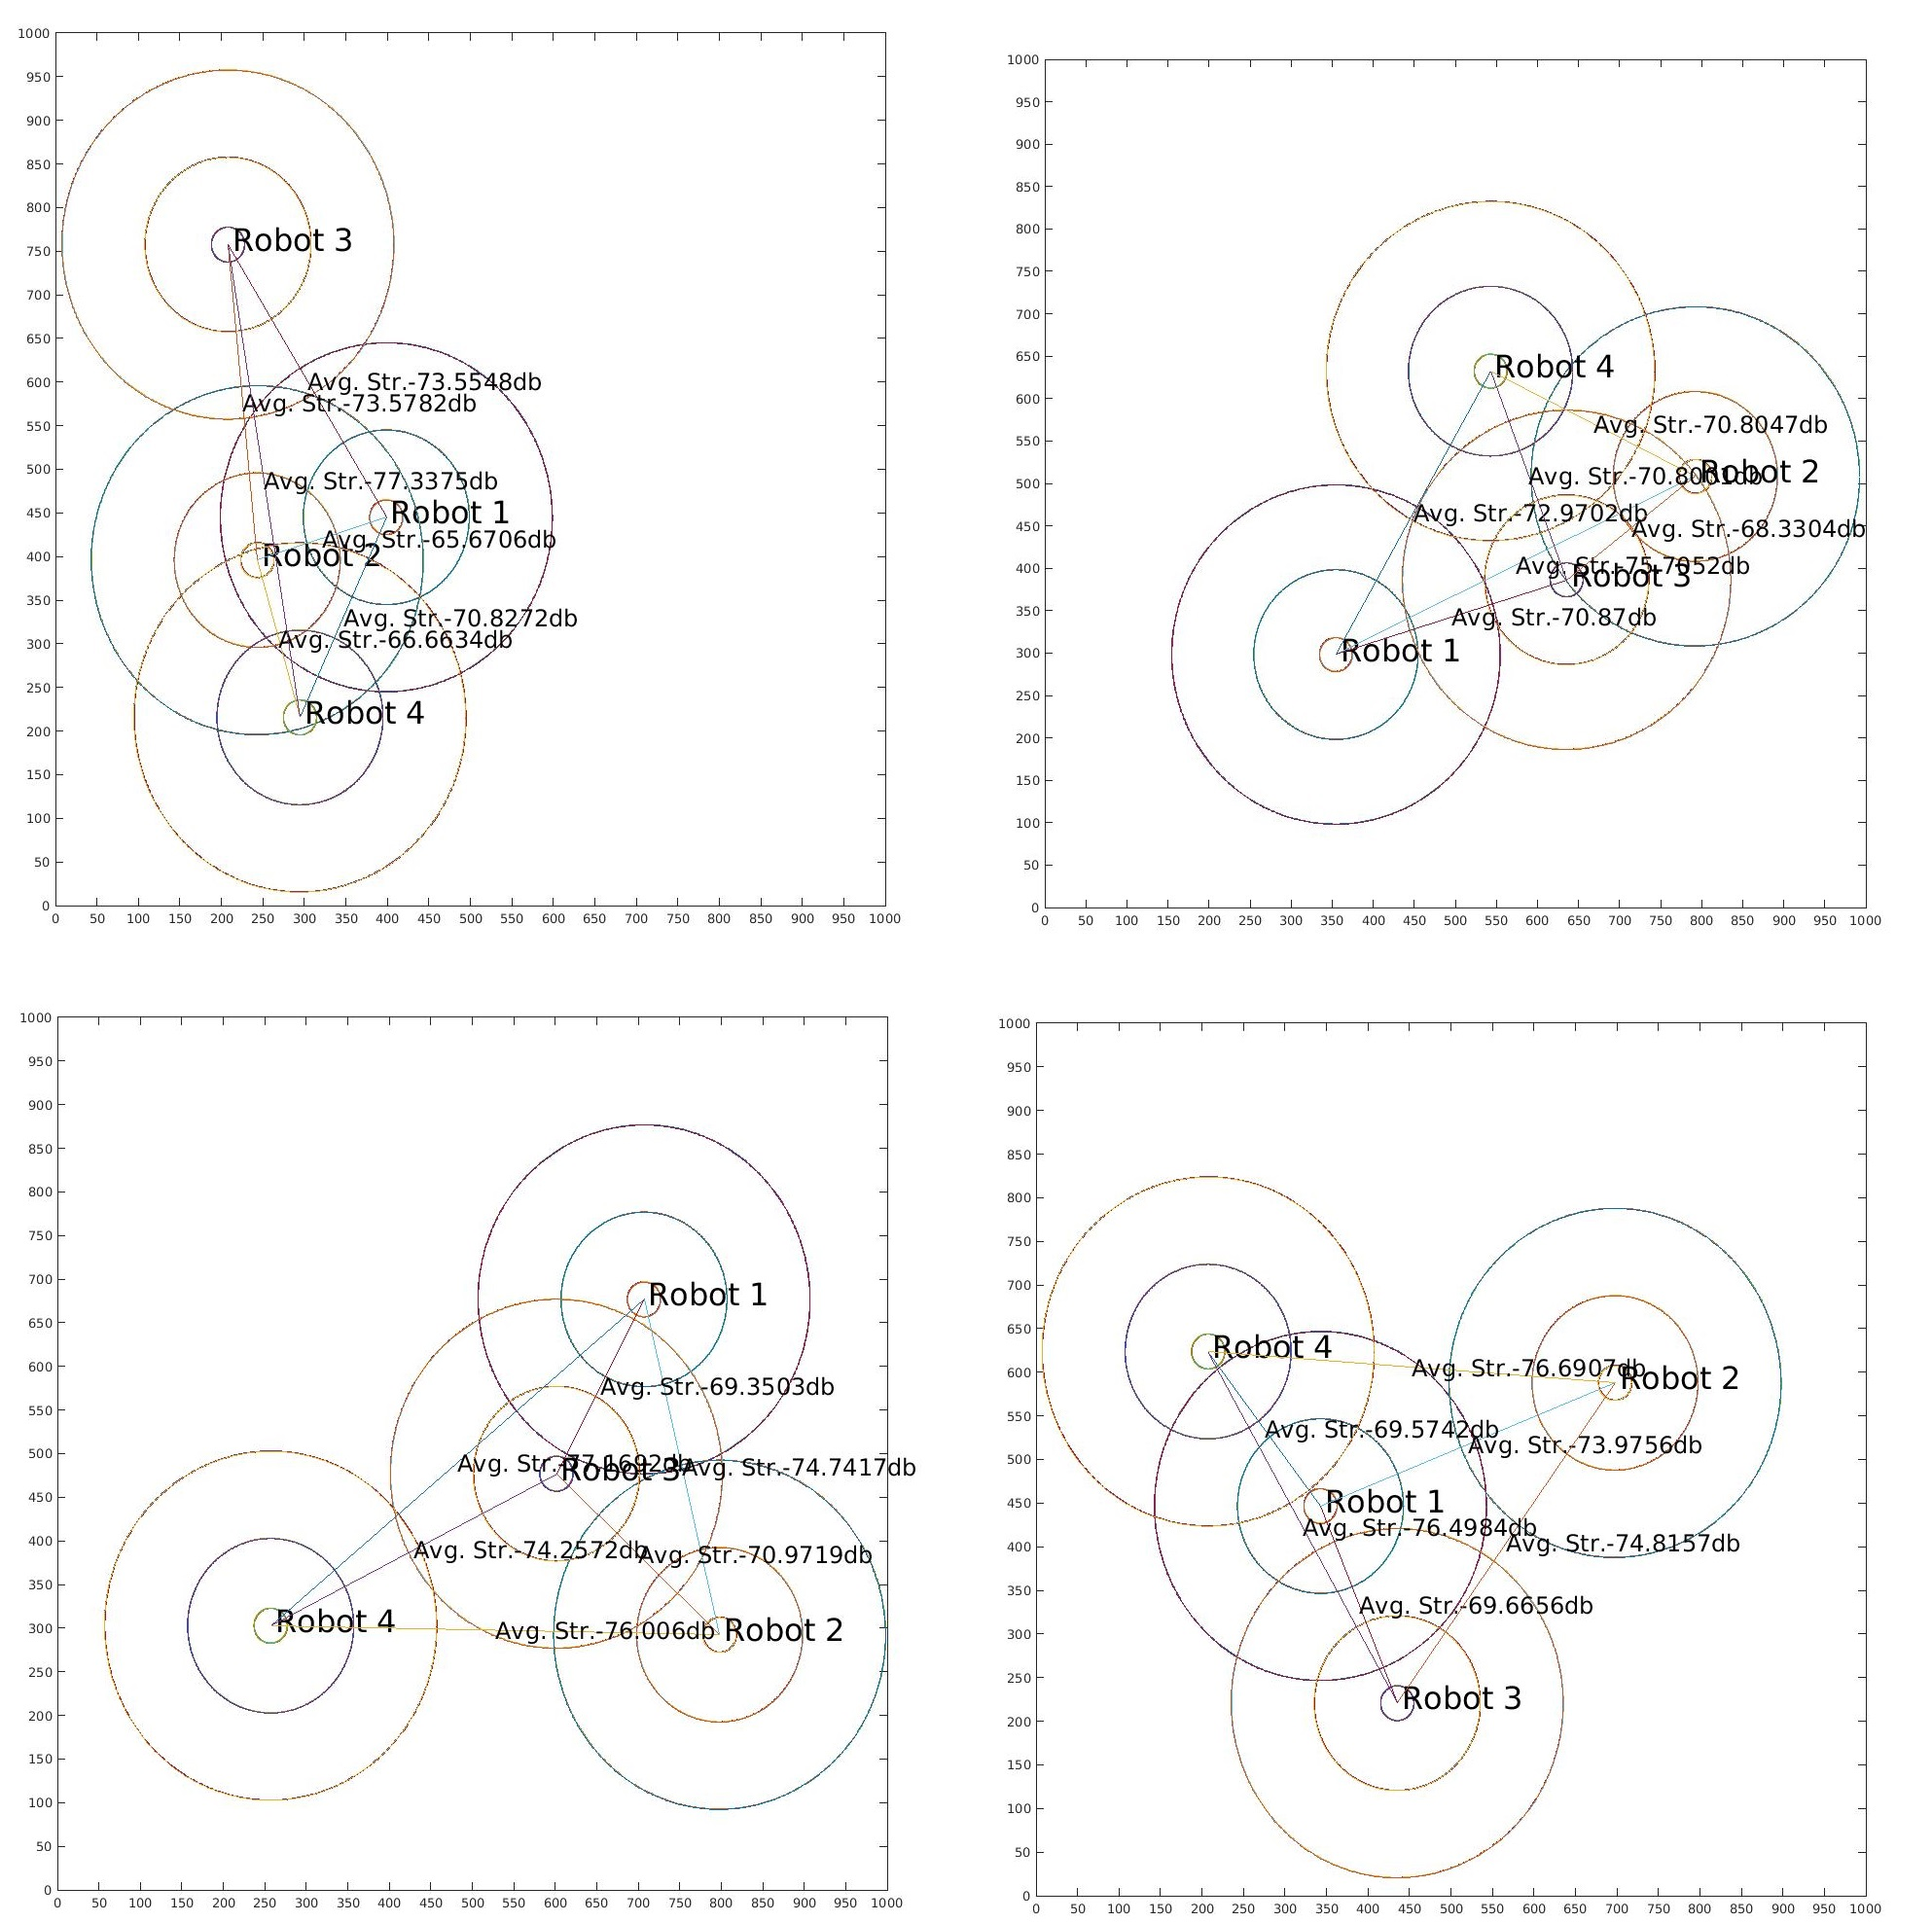
\includegraphics[width=0.4\textwidth]{simulation0}
	\caption{Four sample simulations}
	%\label{fig1}
	\end{figure}
	
\begin{figure}[ht]
	\centering
	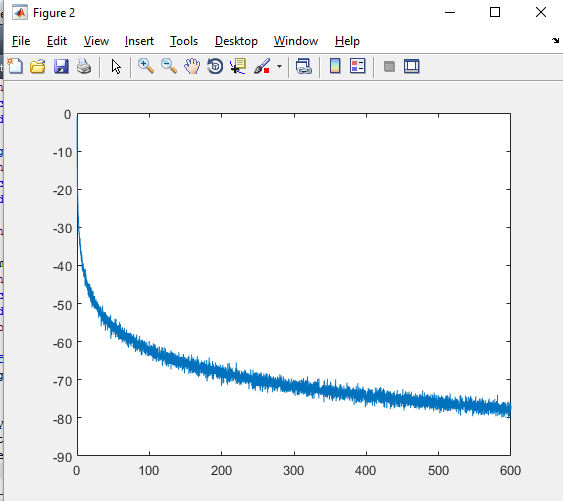
\includegraphics[width=0.4\textwidth]{simulation5}
	\caption{Power vs. Distance}
	%\label{fig1}
	\end{figure}
	
\par
	To have a better understanding of DOA pmuisc function, we implement angle\_ gui.m file to show the simple version of the MUSIC algorithm. Since every robot has four antennas, the receiving signal will be a $1 * 4$ matrix of four signal strength from these antennas. We obtain DOA by applying pmuisc function to the signal matrix.\\
    \begin{figure}[ht]
	\centering
	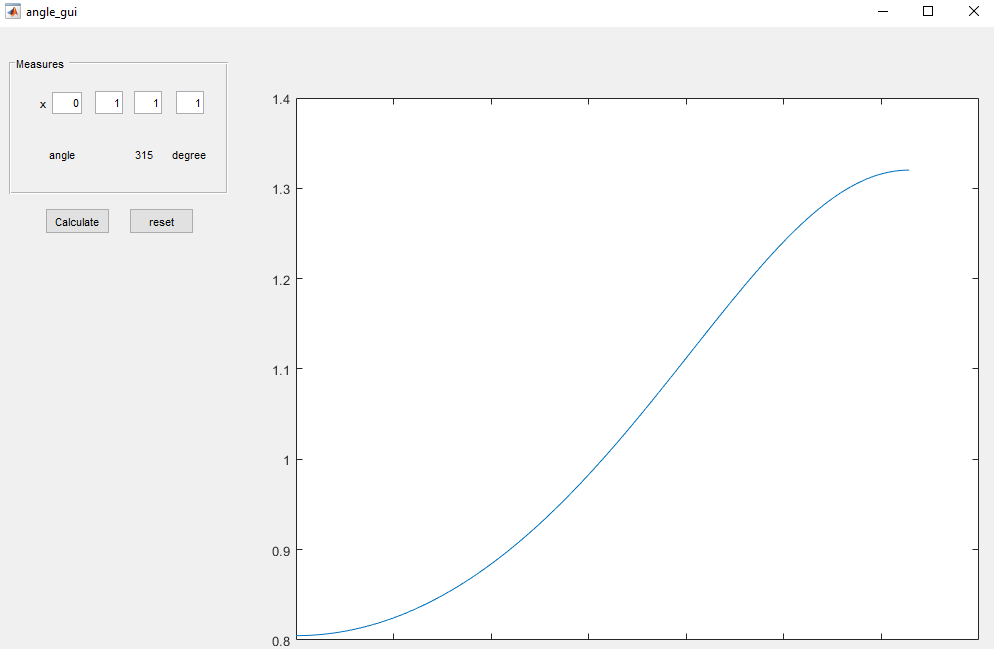
\includegraphics[width=0.4\textwidth]{gui}
	\caption{Four sample simulations}
	%\label{fig1}
	\end{figure}


\subsection{Applying a gathering algorithm}
\par
A network of multiple robots needs to gather robots in the communication range. When multiple robots are placed randomly in a field, the robots firstly need to gather each other until each robots of the network in within the communication range of another robots. A gathering algorithm is applied based on DoA and RSSI acquired from antennas of a robot.
\par
This algorithm is based on the Divide and Conquer algorithm, which firstly group adjacent robots and merge the groups until there is only one big group that covers the all robots in the network. The steps below is used to implement this algorithm. Each robots has four variables: the number of a group a robot belongs to, the number of a robot that the robot is following and moving towards, a mark if the robot is a leader of the group, and a mark that the variables mentioned before, excepts the first one, will not change.

\begin{enumerate}
	\item Select one robot as a root of a network. This root robot is marked as not following any robot and not changing, meaning that the root always holds its position. All robots are not given a group.
	\item Acquire RSSI and DoA. Each robots will follow the a robot that has the strongest RSSI and is not in the same group. The robots marks as not change will not change a following robot.
	\item Move robots towards a following robot for a unit time. If a robot is within a communication range of a following robot, the robot will not move during the unit time. Also, if these adjacent robot are not in any group yet, group them and one robot become a leader and the other robot will follow the leader and is marked as not changing.
	\item If one of the two adjacent robots is in a group and the other robot is not in a group yet, merge them and the robot was not in a group will follow the merging robot and is  marked as not changing.
	\item If the two adjacent robots are in different group and one robot is a leader of a group, the leader robot and the robots in the leader's robot will merge into the adjacent group and the leader robot will loose leadership, follow the adjacent robot and be marked as not changing.
	\item Repeat from step (2) until all robots belongs to the root's group.
\end{enumerate}

\par
With this algorithm, the randomly places robots gather together as seen in the following figure.
	
\begin{figure}[ht]
	\centering
	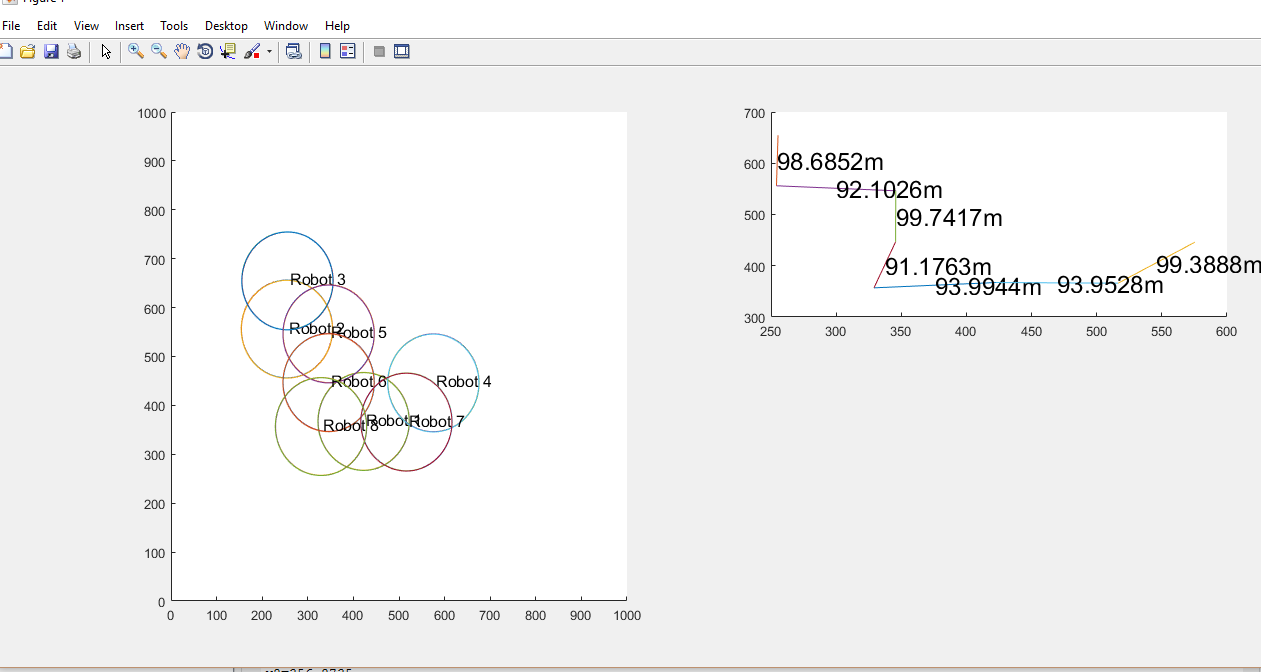
\includegraphics[width=0.5\textwidth]{sample}
	\caption{Simulation sample}
	%\label{fig1}
	\end{figure}


\subsection{Coverage Area(2-D)}
\par
When robots are gathering together within their communication range, we can evaluate the coverage area of the robot network 
system. The ideal maximum range is when each robot's center is located on the edge of other robot's communication range with the first three leading robots forms triangle group like the following graph.
\begin{figure}[ht]
	\centering
	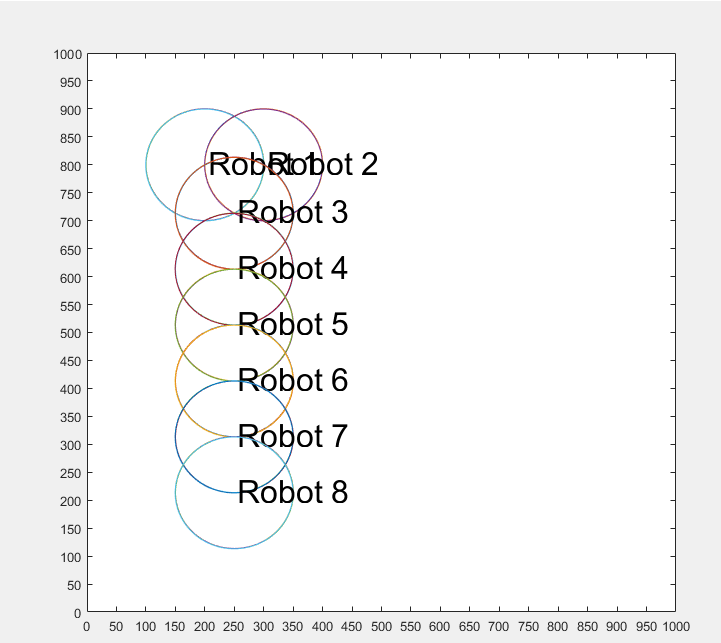
\includegraphics[width=0.4\textwidth]{ideal}
	\caption{Ideal coverage}
	%\label{fig1}
	\end{figure}
	
The geometrical result of ideal area is 1.6058e+05 square meters over 1000*1000 square meters moving area. However, the simulation coverage area is always smaller than ideal area.
The following graph is one of the example of simulation. Eight robots are gathering together and the right graph is their 
topology graph. 

Since geometrical result is too complicated to calculate when simulation could have so many shapes, we decide to calculate the area of simulation area by Monte Carlo method, a broad class of computational algorithms that rely on repeated random sampling to obtain numerical results. we can simply calculate the number of random points located in coverage area over total number of points in moving area times the moving area. To get accurate coverage area, we apply 1000 million random points. The result is 1.5883e+05 square meters. So the coverage difference between ideal and simulation is 1.09 \%.


